As this thesis is a completely new project we will need to build an architecture from the ground up.
Since the main focus of this thesis is visualisation and planning, we aim to provide a realistic feeling experience without being unnecessarily complex.
This means that while our main goal is surgery simulation, we do not focus on realistic physical behaviour of tissue.
The following data will be kindly provided by the OMFS in UHA:
\begin{itemize}
    \item Imaging acquisition
    \begin{itemize}
        \item CT/CBCT scans, MRI scans...
        \item provided by the UHA
    \end{itemize}
\item Image processing
    \begin{itemize}
        \item Apply techniques to segment tissue from scans
        \item Create three-dimensional objects from segmented data
        \item Export data into conventional three-dimensional objects which can be used in the application
    \end{itemize}
\end{itemize}

Furthermore, following key components will be designed and developed for this thesis to give an immersive experience:

\begin{itemize}
    \item Virtual operating room
        \begin{itemize}
            \item Based on real locations in the UHA
            \item If possible, designed via photogrammetry
        \end{itemize}
    \item Provide an interaction system where the user can:
        \begin{itemize}
            \item Freely move around
            \item Interact with virtual model of patient:
                \begin{itemize}
                    \item Magnify and reset to original
                    \item Project another copy of the initial model for comparison
                    \item Set cutting planes
                    \item Mirror at symmetry line
                    \item Simulate cuts including depth by drawing
                    \item Measuring of the following attributes:
                        \begin{itemize}
                            \item distance between two points
                            \item surface / volume area
                            \item angle
                        \end{itemize}
                    \item Transparancy slider for segmented tissue
                    \item Select which tissue to view
                \end{itemize}
            \item Grab surgical instruments
            \item Use instruments for intended operational procedures (drilling, sawing\dots)
            \item Start, undo, save recording movements of currently selected instrument 
            \item Start screen capture (Photo, Video)
        \end{itemize}
    \item Surgical Instruments and materials
        \begin{itemize}
            \item Create realistic virtual objects from real physical instruments and materials which are used in the oral and maxillofacial department of the UHA
            \item Mechanism to plan and view procedures in relation to the patient including:          
                \begin{itemize}
                    \item Angle of the instrument
                    \item Movements including direction of the instrument
                    \item Depth of the instrument if patient was penetrated
                    \item Markings on the patient
                    \item Inform if critical tissue was penetrated
                \end{itemize}
            \item Mechanism to start, stop, redo recordings of procedures for each instrument
        \end{itemize}
    \item Provide an interface to the augmented reality application:
        \begin{itemize}
            \item The user should be able to view all necessary patient data
            \item The user should be able to view screen captures
            \item The user should be able to load planned procedures in both applications by using an agreed format
        \end{itemize}
\end{itemize}

\begin{figure}[ht!]
    \centering
    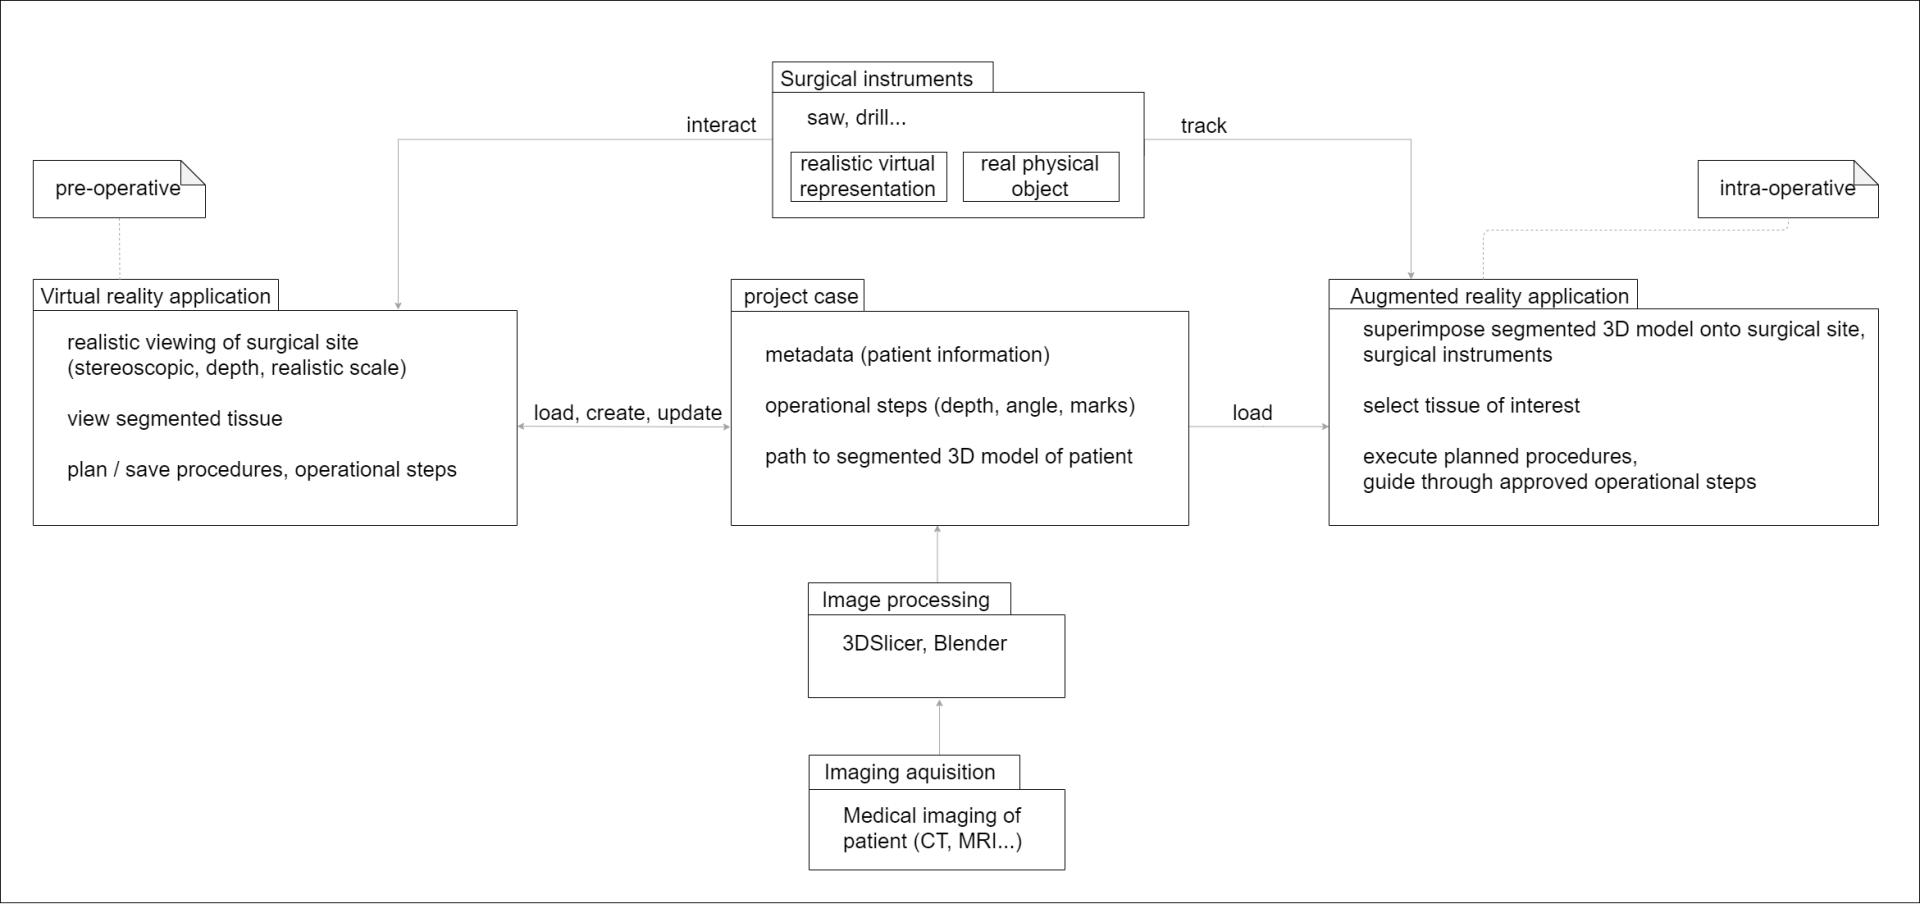
\includegraphics[width=\linewidth]{images/project_plan.png}
    \caption{\label{fig::ProjectPlan} A simplistic view of the architecture.}
\end{figure}

The first step in realizing these requirements is to develop a software architecture with an interface to the augmented reality application in mind.
Since this is a bi-directional data exchange which does not need to be real time, one obvious approach would be to use a simple object notation language such as JSON.
Different options will be explored and decided upon in the beginning phase of the thesis.
However, it is import that we do not have to rely on each other to develop an interface.
To accomplish this, we will agree upon a simple interface before starting the projects.
Hence, we will be able to develop the applications completely independant of each other, even though the applications are linked.

After deciding on a software architecture, the next step is to create a virtual operating room and first surgical instruments.
The operation room will be designed after real operation rooms inside of the UHA.
A photogrammetry approach will be evaluated in the hope to give the most realistic experience as possible for surgeons.
Virtual objects will be combined with a scan of the real world to give an interactive and immersive experience.
After the operating room, the focus will be on developing a traversing mechanism which allows for free exploration of the operating room.
Since operating rooms are not too large in general, it should be possible to traverse them in room-scale VR.
However, a teleport function will be added for convenience.
The surgical instruments will either be created in a 3D modelling software or exported in a similar way to how we obtain the segmented patient models from medical imaging.
The full functionality of the instruments will be developed in a later stage, since we will first work on the more important planning tools.

The planning tools will be the most critical part of the thesis, since they have to behave as expected.
There will be a mix of planning tools which are represented by virtual surgical instruments and basic features which will be mostly visualisation assistance.
At this stage, it will be crucial that the UI is as intuitive as possible and does not distract in any way.
Improving the UI however will be a continious effort throughout the thesis, and will hopefully become as intuitive and assisting as possible.

Each of the surgical instruments will have its own planning operations which can be recorded and saved.
Since at this stage, the architecture and format will already be decided, there should not be too much to worry about when implementing this feature.

There are currently no plans to hold a user study, however an expert review by working surgeons is planned to evaluate the usability and percieved realism of the tool.
Additionally, a small questionnaire will be used after surgery to determine if the new tool is prefered over conventional methods.

There are also possible optional features, such as an additional tool to view dicom data directly, which can be included in the scope of the thesis but will be decided upon during the development phase of the thesis and will be dependent on the progression of the core features of the tool.

As of now, a basic prototype is already developed to showcase some of the planned functionality of the application.




